\section{Statistical tools}
\label{chp:sec:stat}
The primary goal of data analysis in particle physics is to test our understanding of particle interactions and to search for new phenomena not accounted by the SM. Statistical concepts help in quantifying the correspondence between theoretical predictions and experimental observations. 
The use of a statistical test in a physics analysis, involving different event types, comes up in different ways: sometimes to carry out measurements and sometimes to make a statement about the existence of a new signal process.
Hypothesis testing addresses the question whether some observed data sample is more compatible with a given theory model or with an alternative one.
Discovery is formulated in terms of a hypothesis test where the background-only hypothesis plays the role of the null hypothesis, $H_{0}$, and the signal-plus-background hypothesis plays the role of the alternative test hypothesis, $H_{1}$. The two hypotheses can be generalised by introducing a signal strength modifier, $\mu$,
which acts as a multiplicative factor to the signal cross section. The null (test) hypothesis is recovered for $\mu=0$ (1). In the search for the $t\bar{t}H$ process, the SM without the Higgs boson is considered the background-only hypothesis, while the signal-plus-background hypothesis includes the Higgs boson as signal. Searches for BSM signatures include the SM Higgs boson in the background model.\\ \indent The claim of discovery is a statement that the data are incompatible with the background-only hypothesis.  Testing an hypothesis means to quantify the agreement between the outcome of a measurement and the predictions coming from that hypothesis using a test statistic. From the test statistic a $p$-value, $p_{\mu}$, is the probability to obtain a value of the test statistic as large or larger than the one observed, assuming a model with signal strength $\mu$. If this $p$-value is less than some specified value $\alpha$, usually referred to as the power of the test, the model is rejected. The $p$-value is often translated into an equivalent quantity called the Gaussian significance, $Z$, defined as the number of standard deviations that correspond to an upper-tail probability of $p$-value for a Gaussian-distributed variable. The definition of significance and $p$-value are shown in figure \ref{fig:dat:stat:pvalue}. The convention to exclude a new process ($\mu=1$) is that $p$-value should be less than $5\%$ but to claim a discovery (excluding $\mu=0$ hypothesis), instead, it is common to set the $p$-value to a very low value of $2.9\times 10^{-7}$ that corresponds to a significance $Z$=5. 
Setting the $p$-value to the value of the power of the test ($p_{\mu}=\alpha$) and solving for $\mu$ provides the highest and the lowest $\mu$ that are not excluded (upper and lower limits respectively) at a confidence level equal to $1-\alpha$. 


\bfig[htb!]
\centering
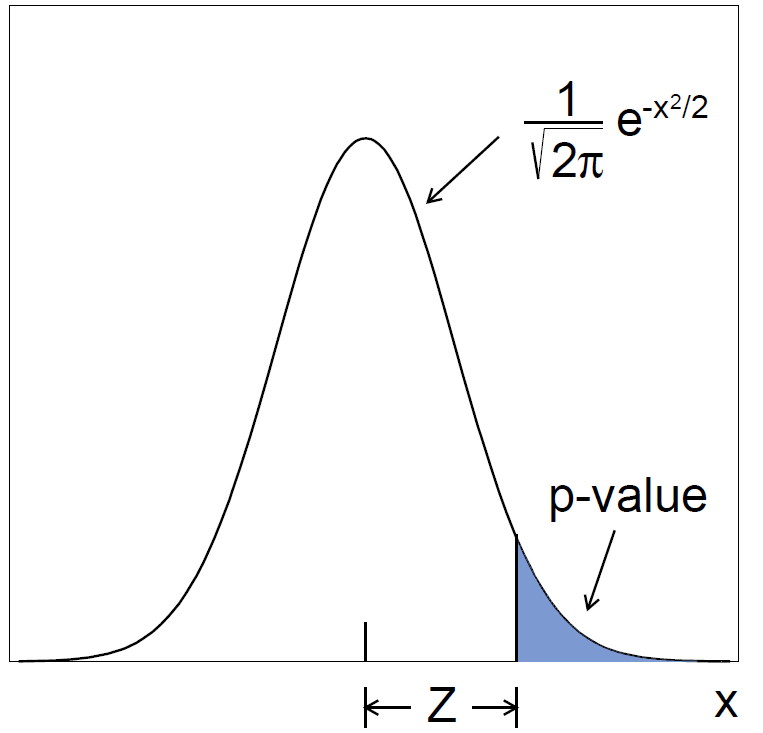
\includegraphics[width=0.4\textwidth]{figures/Datasamples/pvalue.png}
\captionsetup{width=0.85\textwidth} \caption{\small Illustration of the definition of $p$-value and significance $Z$.}
\label{fig:dat:stat:pvalue}
\efig

\subsection[$CL_{s}$ procedure]{\boldmath{$CL_{s}$} method}

In case the distributions of a test statistic, $q_{\mu}$, for signal and background are very close (``low sensitivity''), the $p$-value can reject a model even if there is no enough sensitivity due to downwards fluctuations in the observed data. With $\alpha$ set to $5\%$ a model every twenty will be excluded even if there is no sensitivity. A solution to this problem is the $CL_{s}$ method \cite{Junk:1999kv}, which in case of low sensitivity alters the threshold to reject a model by defining:

\be
CL_{s}= \frac{p_{\mu}}{1-p_{0}},
\ee 

\noindent where $p_{0}$ is the $p$-value for the background-only hypothesis. In case of low sensitivity if $p_{\mu}<\alpha$ the quantity $1-p_{0}$ will be small as well leading to $CL_{s}$ value greater than $p_{\mu}$ such that the model will not be rejected (see figure \ref{fig:dat:stat:cls}). For searches at the LHC, the $CL_{s}$ value is used instead of $p_{\mu}$ to set upper limits. If $CL_{s} < 0.05$, the signal-plus-background hypothesis with a signal strength $\mu$ is excluded at $95\%$ confidence level.

\bfig[htb!]
\centering
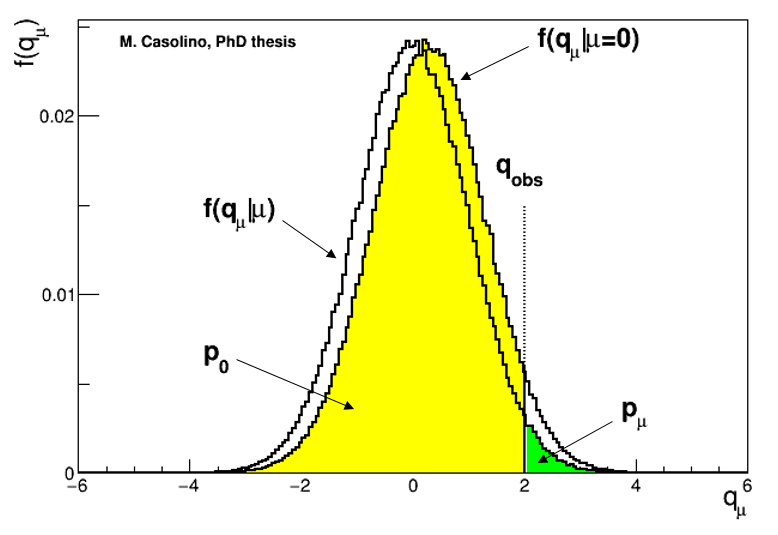
\includegraphics[width=0.5\textwidth]{figures/Datasamples/lowsensitivity.png}
\captionsetup{width=0.85\textwidth} \caption{\small Illustration of the ingredients for the $CL_{s}$ limit in case of low sensitivity.}
\label{fig:dat:stat:cls}
\efig


\subsection{Profile likelihood ratio}

The data in each bin of each distribution are expected to follow a Poisson probability distribution around the expected mean of $\mu s+b$, where $s$ and $b$ correspond to the number of expected signal and background events, and $\mu$ is the signal strength modifier. A likelihood function is obtained from the probability of data given a certain hypothesis. Therefore, the likelihood for the observed data produced by this model is:

\be
L(\mu)=\displaystyle\prod_{i=1}^{\rm bins} \frac{\mu s_{i}+b_{i}}{n_{i}!} e^{-\mu s_{i} +b_{i}}.
\ee

To establish the existence of the signal process tests of different hypothetical values of $\mu$ should be performed. To maximise the probability of a discovery the test of the background-only ($\mu=0$) hypothesis should have as high power as possible. According to the Neyman-Pearson lemma, the maximum power is achieved by basing the test on the likelihood ratio $L(\mu)/L(\mu=0)$, or equivalently on the statistic:

\be
q_{\mu}=-2 \ln \frac{L(\mu)}{L(\mu=0)}.
\ee

\noindent Thus the best estimate for $\mu$ is obtained minimising this statistic, which means to maximise the likelihood for the signal-plus-background hypothesis.\par
The number of background in events is usually affected by uncertainties in the form of systematic and statistical errors. A more realistic approach consists in including the systematic uncertainties directly in the definition of the likelihood through a suitable set of continuous parameters $\theta$, referred to as nuisance parameters (NPs), that parametrise the effect of each uncertainty on the signal and background predictions. As a net effect, the various terms in the likelihood acquire a dependence on $\theta$; varying the values of the NPs allows to modify both the shape and normalisation of the signal and background predictions. The maximisation of the likelihood leads to adjustments in the NPs in order to improve the agreement of the expectation with the observed data. The NPs are characterised by a probability distribution function (pdf) $\rho(\theta)$, encoding the information about its best estimate and width, which is related to the size of the uncertainty. The pdfs for each systematic uncertainty are determined beforehand by auxiliary measurements. The pdf is also included in the likelihood and is usually referred to as penalty term or prior on $\theta$. The prior distribution for NPs is commonly assumed to be a Gaussian but other distributions (log-normal, gamma) could be more suitable in specific cases. This description of the priors is based on the absolute values of the NP and their uncertainties, and understanding the fit result becomes very difficult since it requires the knowledge of the pre-fit values for each NP. In order to simplify the analysis, all NPs are redefined in order to be centred at zero and with a width of one. The nuisance parameters are unknown parameters that need to be determined by the fit. This approach allows the data under study to potentially improve the initial knowledge of systematic uncertainties obtained from external inputs to the analysis.  In case the data are not particularly sensitive to a given source of systematics, the constraint term in the likelihood ensures that the nuisance parameter stays at 0 and its error is dominated by the input uncertainties. On the other hand, the fit procedure could shift (pull) a nuisance parameter to achieve a better data/MC description or, at the same time, produce a reduction (constraint) of the error of the nuisance parameter with respect to its initial value. This usually happens when the large effects of a particular systematic uncertainties are not supported by the available data statistics. Furthermore, during the likelihood maximisation process, correlations can be established among nuisance parameters that have similar effects in the regions considered by the fit, which further aids in the reduction of the final effect of the total systematic uncertainties.\par
Using the pdf for the NPs we can write the likelihood as:

\be
L(\mu,\theta)=\displaystyle\prod_{i=1}^{bins} \frac{\mu s_{i}+b_{i}}{n_{i}!} e^{-\mu s_{i} +b_{i}} \displaystyle\prod_{k=1}^{NPs} \rho(\theta_{k}).
\ee

\noindent The profile likelihood is defined as:

\be
L_{p}(\mu)=L(\mu,\hat{\hat{\theta}}(\mu)),
\ee

\noindent where $\hat{\hat{\theta}}(\mu)$, known as profile values of the NPs $\theta$, are the values that maximise $L(\mu,\theta)$ for the fixed value of $\mu$.

The test statistic used at the LHC and in this dissertation is based on a likelihood ratio to maximise the power of the test. Specifically, it is a profile likelihood ratio \cite{Cowan:2010js} defined as:

\be
q_{\mu}=-2 \ln\lambda(\mu)=-2\ln\frac{L_{p}(\mu)}{L(\hat{\mu})},
\ee 

\noindent where $\hat{\mu}$ is the value that globally maximises the likelihood. The profile likelihood ratio $\lambda(\mu)$ lies between 0 and 1, with values of $\lambda$ close to 1 implying good agreement between the data and the hypothesised value of $\mu$.\par
From the test statistic a $p$-value can be computed, giving the probability that the observed data originates from the considered hypothesis:

\be
p_{\mu}=\int_{q_{\mu,{\rm obs}}}^{\infty} f(q_{\mu}|\mu,\theta)dq_{\mu},
\ee

\noindent where $q_{\mu,{\rm obs}}$ is the observed value of the test statistic in data and $f(q_{\mu}|\mu,\theta)$ denotes the pdf of $q_{\mu}$ assuming the hypothesis $\mu$. The computation of background-only quantities such as $p_{0}$ are just special cases with $\mu = 0$.

For sufficiently-large data samples the Wilk and Wald theorems \cite{WaldApprox} demonstrate that the distribution of the pdf for the test static $q_{\mu}$ approaches an asymptotic form related to the chi-square distribution with one degree of freedom. 
The test statistic in this approximation has a form:
\be
q_{\mu}=-2 \ln\lambda(\mu)=\frac{(\mu-\hat{\mu})^{2}}{\sigma^{2}}+\mathcal{O}(1/\sqrt{N}),
\ee

\noindent where the fitted strength parameter $\hat{\mu}$ follows a Gaussian distribution with a mean $\mu$ and standard deviation $\sigma$, and $N$ accounts for the data sample size. This formula requires knowing the variance of the maximum likelihood estimate of $\mu$, which can be estimated from an artificial dataset referred to as the Asimov dataset \cite{Cowan:2010js}. The Asimov dataset is defined as the one where the pseudodata is equal to the expectation value, i.e. to the sum of background predictions. An important advantage of using the profile likelihood ratio is that its asymptotic distribution is independent of the nuisance parameters. For the searches described in this dissertation the asymptotic approximation \cite{Cowan:2010js} is used in order to compute the relevant $p$-values.
